\documentclass{article}
\usepackage[utf8]{inputenc}
\usepackage{graphicx}
\usepackage{subcaption}
\usepackage[export]{adjustbox}
\usepackage{wrapfig}
\title{Extrapolating NBA Career Trajectories From Rookie Year Stats}
\author{Akash Kumar(ajk279) and Pranav Darbha(pd353)}
\date{\vspace{-5ex}}
\begin{document}

\maketitle
\clearpage
\section{Introduction}
In the annual NBA Draft, 60 players from American universities and other leagues around the world are chosen in the hope that they can be strong players in the world's most competitive basketball league. The volatility of the rookie season can make it difficult to predict how a player will perform further into their NBA career. There are those who succeeded in their first taste of the NBA and never looked back like LeBron James, those who have continually regressed since that first year like Michael Carter-Williams, and those who were quiet at first but broke out in a big way like Kawhi Leonard. With the value of contracts constantly increasing, the decision regarding how much money and time to invest into these rookies has gotten increasingly important. Being able to accurately predict the trajectory of these players' performances has become one of the most indicative signs of a championship-caliber organization in the NBA.

With the plethora of NBA data available for draft classes throughout the years, we wanted to predict the performance of 2016-17 Rookies in the upcoming season. We used datasets from www.basketball-reference.com containing player statistics from 2010 onwards as well as NBA 2K ratings to measure the overall capability of a player. From basketball-reference, we used both traditional metrics like points, rebounds and assists (per 36 minutes to account to avoid penalizing players for not getting playing opportunity) as well as advanced statistics like Player Efficiency Ratings and Value Over Replacement Player. We collected this data from the players' rookie years and used it to predict their NBA 2K ratings 3 years down the line, an important benchmark in a player's career because it is after this season that they start their next contract if they receive one. We believe 2K ratings are accurate indicators of overall skill because they are meticulously developed to take into account all aspects of a player's game. They are also widely accepted as the video game franchise routinely sells over 10 million copies each year. We decided to use this rating from a model design perspective because we wanted a quantitative way to predict a player's overall future potential rather than classifying them into tiers based on awards or simply predicting specific statistics. Once we built our predictive model, we evaluated its performance by looking at the stats of the 2016-17 Rookies in their fourth NBA season, which began recently. NBA 2K ratings have gone through many iterations of updates this season as they are updated biweekly, and we used these updated ratings to evaluate the models.
\section{Data and Preprocessing}
As was previously mentioned, we collected a mix of advanced and traditional statistics for each player's rookie and fourth year seasons from basketball-reference.com. Our models are only trained on the players' rookie year statistics to predict the 2k rating, but we collected the statistics for the fourth year as well for us to reference. Figure 1 shows the features that were used and the correlation between them. 
\begin{figure}[htp]
    \centering
    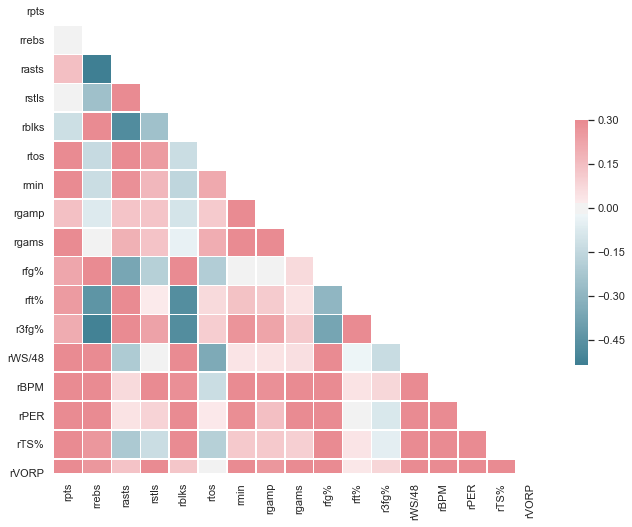
\includegraphics[width=10cm]{feature_heatmap.png}
    \caption{Heatmap showing our features and the correlations to the other features}
\end{figure} 

Our first intuition was to manually label each player by classifying them into 5 tiers. These tiers loosely corresponded to "Bench player", "Rotation player", "Starter", "All-Star caliber", and "All-NBA caliber". We manually labelled them by looking at the accolades and stats they had accrued in their first four years. We initially represented these labels with one-hot vectors, but we saw poor performance from the models because the overwhelmingly high number of Tier 1 players gave us high accuracy models that misclassified many players as Tier 1. We then changed our labels using the encoding style normally used for ordinal data that was shown in class. This change in encoding did not make much of a difference, however, which led to us pivoting and using a regression approach with the NBA 2k ratings rather than a multi-class classification based on subjective labels. We did however revisit the classification idea later on by instead creating groups of 2K ratings. To collect this data we visited a variety of sites that tracked these ratings and added the ratings to the dataset.
\section{Model Development}
As our problem involved predicting integer ratings, we felt that a regression was the best kind of model to fit on our data. We made sure to split up our data randomly into training and test sets with 20 percent of the data in the test set. This provides us with a way to check if our models are accurate and if they are overfitting or underfitting. We made sure to also scale our features in order to make up for the order of magnitude difference between statistics such as points and VORP. We then fit four different kinds of regression models taking in the rookie statistics as input features and outputting the predicted 2k rating. These were linear regression without regularization, polynomial regression without regularization, lasso regression, and ridge regression.

\begin{figure}[h]
\begin{subfigure}{0.5\textwidth}
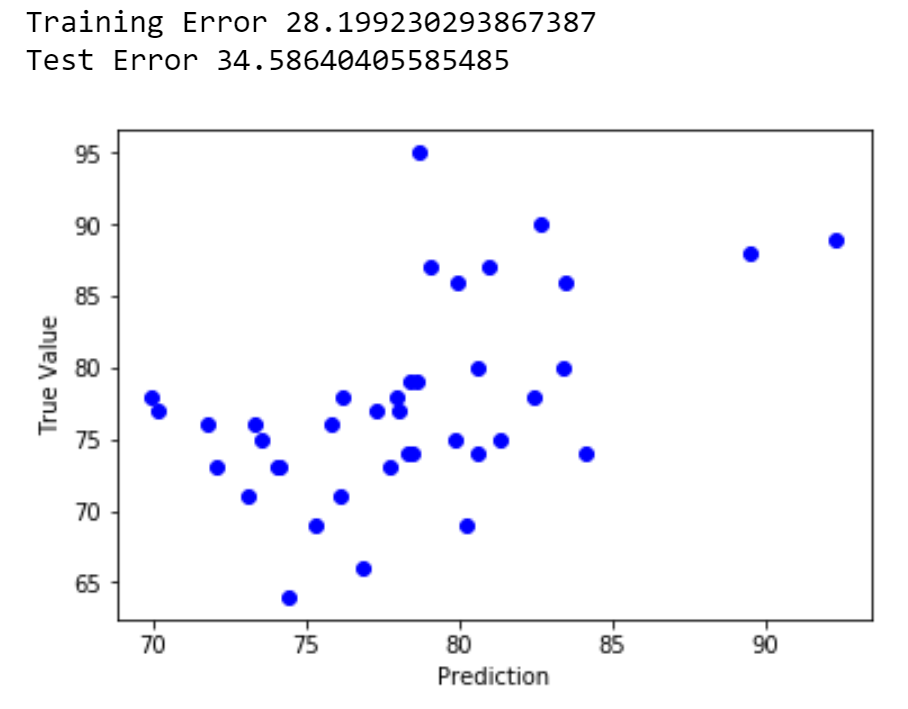
\includegraphics[width=0.9\linewidth]{nbalinreg.png} 
\caption{Linear Regression}
\end{subfigure}
\begin{subfigure}{0.5\textwidth}
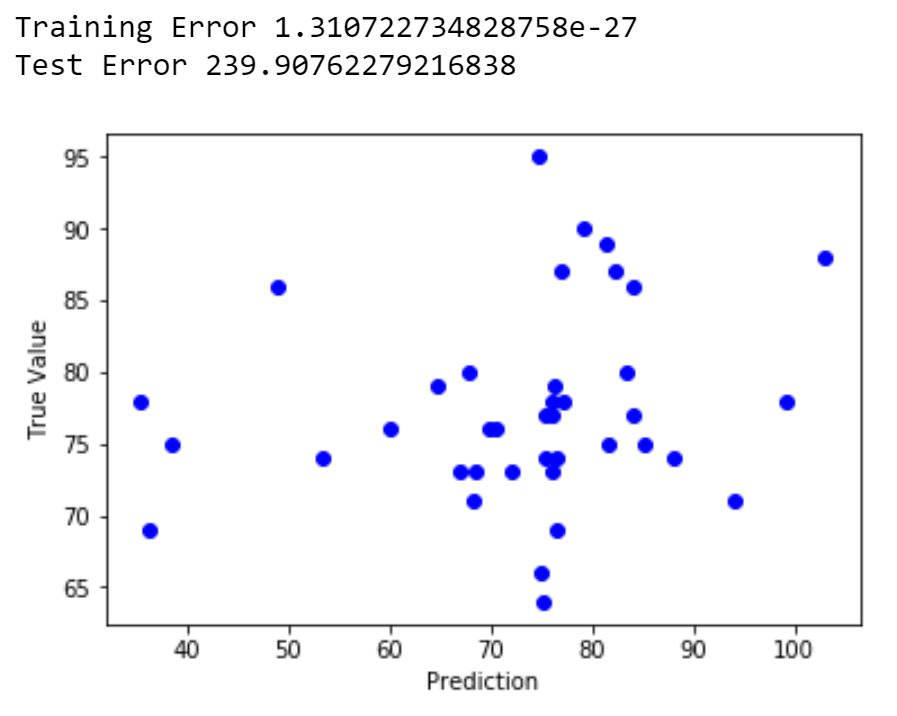
\includegraphics[width=0.9\linewidth]{nbapolyreg.png}
\caption{Polynomial Regression}
\end{subfigure}
\end{figure}
\begin{figure}[h]
\begin{subfigure}{0.5\textwidth}
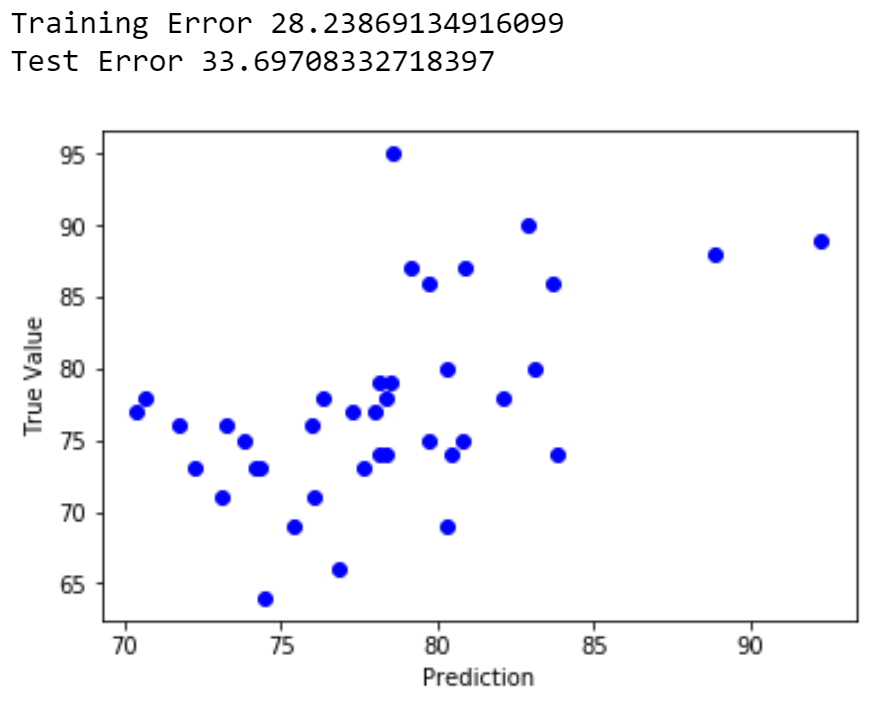
\includegraphics[width=0.9\linewidth]{nbaridgereg.png} 
\caption{Ridge Regression}
\end{subfigure}
\begin{subfigure}{0.5\textwidth}
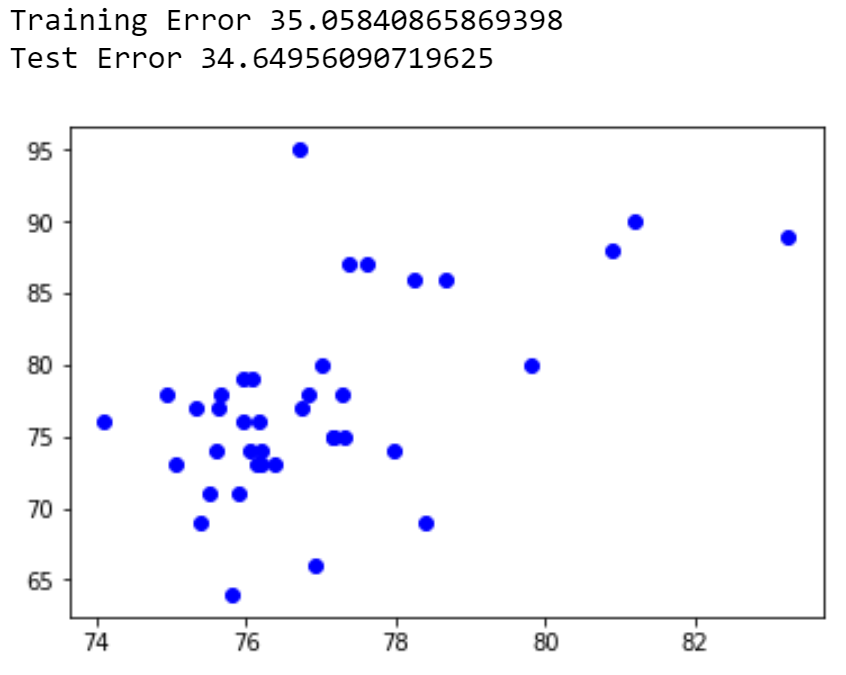
\includegraphics[width=0.9\linewidth]{nbalassoreg.png}
\caption{Lasso Regression}
\end{subfigure}
\end{figure}
Linear Regression and Ridge Regression appeared to be our two best models in the preliminary analysis. Both had mean squared training error around 28 and mean squared test error around 34. Ridge improves slightly on the test error at the expense of some training error and Lasso does worse on both fronts. In the context of our model, this error means that our predictions are, on average, around 5-6 rating points off. From these results, we decided to move forward with ridge regression for hyperparameter tuning and also decided to try regularization with polynomial regression, since that could significantly improve the overfitting problem.

In our hyperparameter tuning we wanted to try all possible values of lambda for ridge regression from 0 to 500 and pick the one with the best results. In order to do this, we created a 60/20/20 split between training data, validation data, and test data. We would fit the model itself on the training data, tune the hyperparameter on the validation data and finally check results on the test data. Trying possible values of lambda in increments of 0.05 from 0 to 500 for ridge regression gave us the following results for our best model. We found the best value for lambda to be 29.25 and saw training and test error both around 32, which was an improvement from our preliminary analyses.

Now we also wanted to try polynomial regression with regularization. We decided to try both \(l_1\) and \(l_2\) regularization to compare results and use hyperparameter tuning for each. We also wanted to try multiple degrees of regression and pick the best model across all parameters. The tuning involved the same process of a 60/20/20 split between training, validation and test data. After trying the various possibilities, we ended up having the best results by using degree 2 and \(l_1\) (Lasso) regularization with a regularization parameter of 0.91. We found a training error of around 34 with a test error slightly above 32. This was slightly worse than the results we found from ridge regression, but still an improvement over our preliminary analyses. The graph of predicted vs true values for this model is below.

\begin{figure}[h]
\begin{subfigure}{0.5\textwidth}
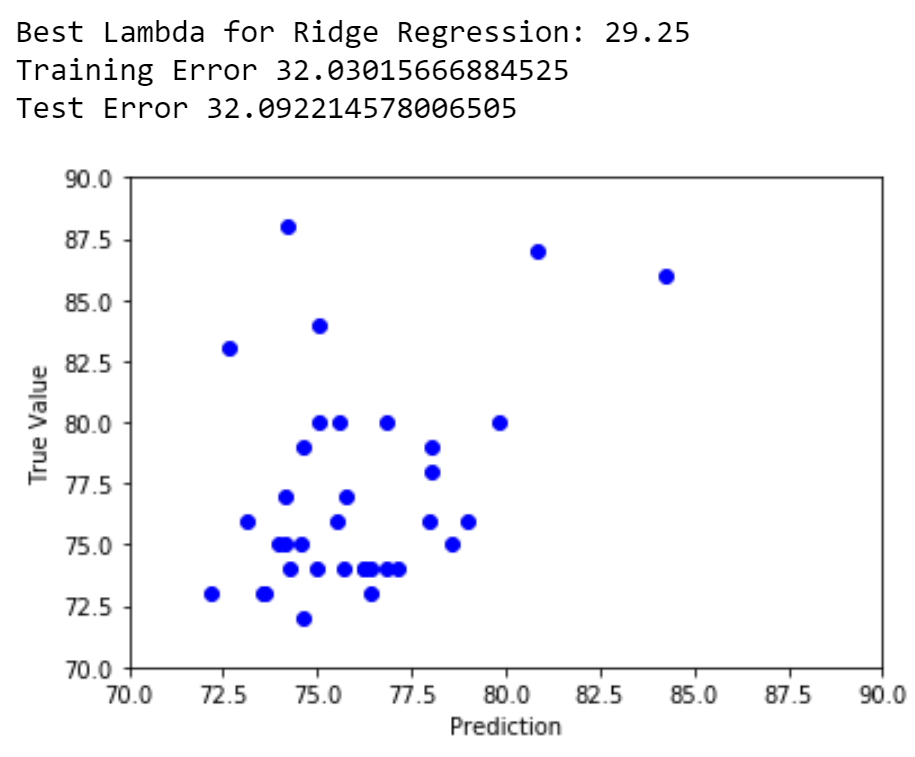
\includegraphics[width=0.9\linewidth]{ridgewithtuning.png} 
\caption{Ridge regression with parameter 29.25}
\end{subfigure}
\begin{subfigure}{0.5\textwidth}
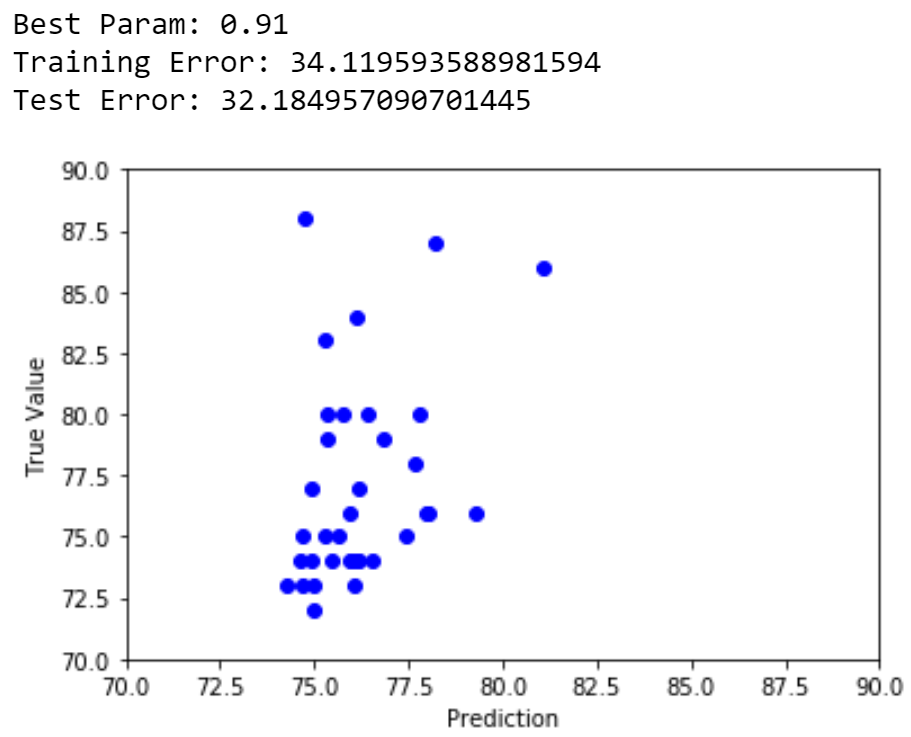
\includegraphics[width=0.9\linewidth]{polyregwithtuning.png}
\caption{Polynomial regression of degree 2}
\end{subfigure}
\end{figure}\\

The mean squared error of our regression models led us to believe that we could accurately predict the ratings of players with a buffer of 5-6 points. With this in mind, we believed that an ordinal classification would be more appropriate for this situation. We modified the outputs to be 5-dimensional vectors, which were formatted as such: \([rating\geq70, rating\geq75, rating\geq80, rating\geq85, rating\geq90\)], where if the Boolean expression was true, the element would be 1 and 0 otherwise. Since this became a classification problem, we tried training classification algorithms to best accomplish this task. We tried to train 5 different logistic regression models which predicted each element of the output vectors since classification algorithms can only predict 0 or 1. We did the same thing with 5 different Support Vector Machines (SVMs). We compared these models to a singular neural network with 1 hidden layer of size 100 that outputs a 5-dimensional vector. The models were evaluated using a test set which was 20\% of the training data. Out of these models, the neural network gave us the best results. The results of running the neural network on the test set are shown in the table below. The column "Pred" refers to the predicted category and "Act" refers to the actual category where the categories were determined by adding the elements of the vector. This means that a category of 0 refers to ratings below 70, 1 refers to 70-74, 2 refers to 75-79, 3 refers to 80-84, 4 refers to 85-89, and 5 refers to ratings 90 and above.
\begin{figure}[htp]
    \centering
    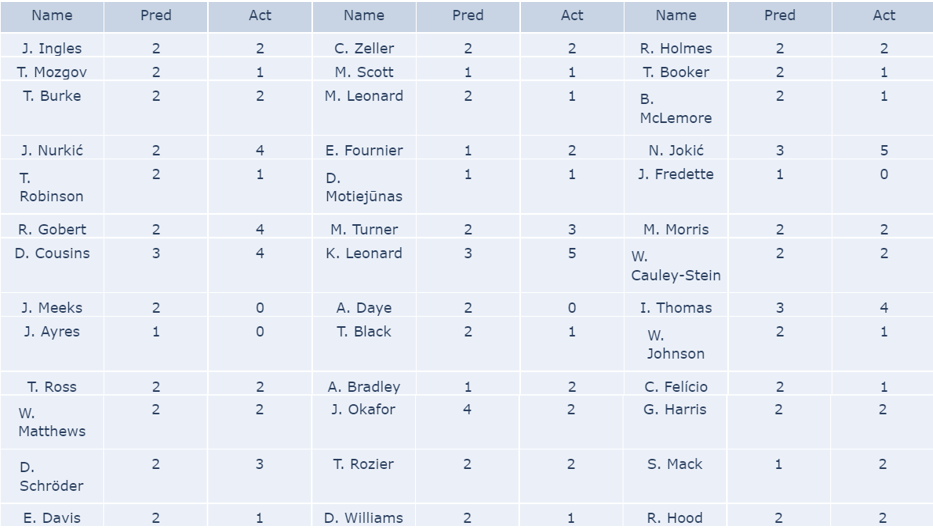
\includegraphics[width=12cm]{category_table.PNG}
    \caption{Table showing the results of our ordinal classification.}
\end{figure}
On average, our classifications were off by 0.846. This is consistent with our earlier regression results which were off by an average of 5-6 points, which corresponds to 1 tier. Doing a closer analysis of our test results shows that we were able to predict everyone's tier within 1 tier, except for a few exceptions. These exceptions include Jusuf Nurkic, Rudy Gobert, Kawhi Leonard, Jahlil Okafor, and Nikola Jokic. These are notable examples as Nurkic, Gobert, Leonard, and Jokic are all examples of players who were not expected to amount to much who developed into super stars or extremely valuable contributors. Their career trajectories were not normal since they progressed so much so fast, which is why our model had trouble predicting their ratings. Okafor is notable for the opposite reason as he was expected to be a great contributor and was given ample opportunity to prove it when he did not deserve those opportunities. After a little over a season, the league began to realize that Okafor was not actually great, and his playing time, statistics, and rating consequently decreased. Since his trajectory was unconventional as well, the model found it difficult to predict his rating based on just his rookie statistics. If we exclude these outliers, our classifications were off by 0.697. From this we can conclude that our model generally does a good job of predicting a player's category in 3 years, but variations in player development trajectories can lead to inaccuracies.
\section{Evaluation on 2017 Rookies}
As we mentioned earlier, we wanted to use our model to predict the ratings of the rookies from the 2016-2017 NBA season from this current year. We attempted to use our models to predict the current ratings of those players, which we got from the most recent ratings update from NBA 2K. 
\subsection{Evaluation Using Regression}
We tried both of our best regression models on the dataset of 2017 rookies. The first model we tried was the Polynomial Regression of degree 2 with \(l_1\) regularization with parameter 0.91. This ended up giving us a mean-squared error of 22.55 which was actually a big improvement from the errors we saw earlier. This means we are off between 4-5 points for each players' ratings rather than 5-6. The graph of predicted vs true values for 2017 rookies using this model is shown below.

We then tried the ridge regression model we developed earlier with regularization parameter 29.25 on the 2017 rookie data. This gave us a mean-squared error of 24.55, again an improvement from the errors this model produced on our older data. The graph for this model on 2017 data is shown below.\\
\begin{figure}[h]
\begin{subfigure}{0.5\textwidth}
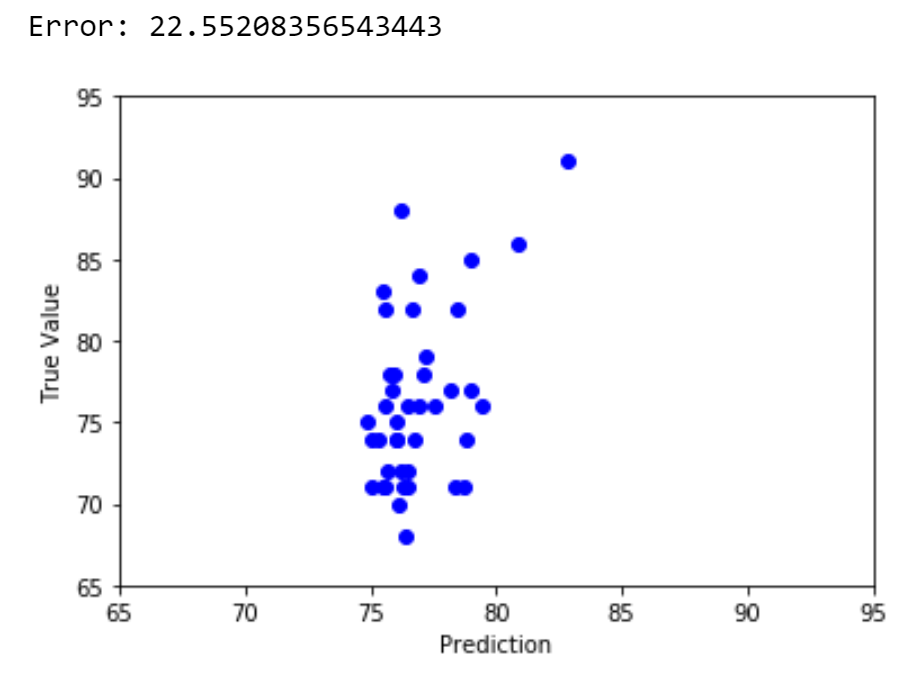
\includegraphics[width=0.9\linewidth]{polyregonlatest.png} 
\caption{Polynomial Regression on 2017 Rookies}
\end{subfigure}
\begin{subfigure}{0.5\textwidth}
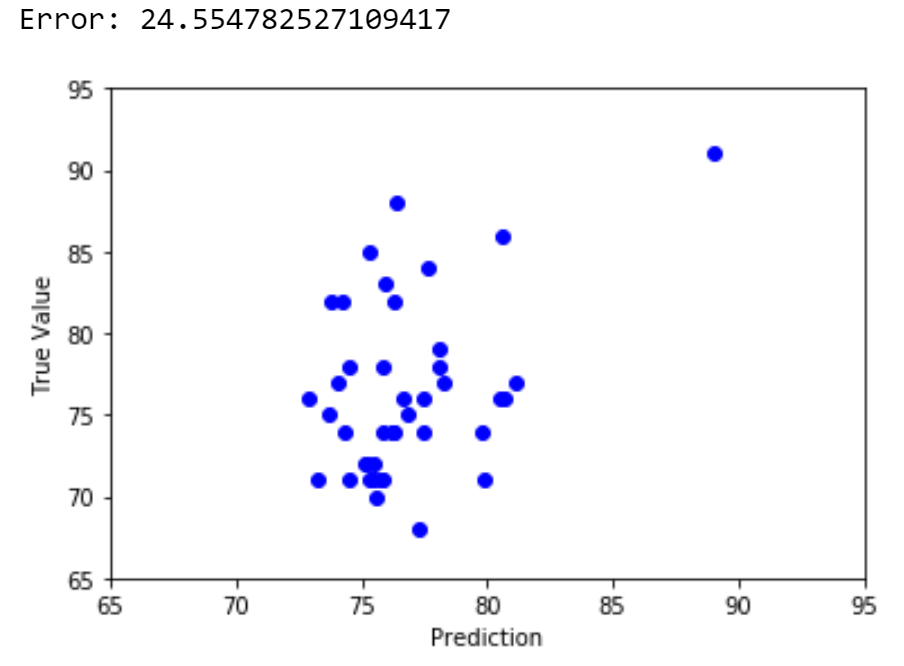
\includegraphics[width=0.9\linewidth]{ridgeregonlatest.png}
\caption{Ridge Regression on 2017 Rookies}
\end{subfigure}
\end{figure}\\
It is difficult to explain precisely why our regression models actually performed better on 2017 data than the data we trained and tested on. We believe the primary reason is that the model generalizes fairly well and the 2017 class produced less outlier prospects than other draft classes. This resulted in far less data with large rating disparities which helped improve our overall mean squared error.
\subsection{Evaluation Using Classification}
Our model of choice for our classification-based approach was a neural network that predicted the ratings-based category of the NBA player. When ran on the dataset of 2017 rookies, our results were slightly worse than the test set results earlier. The results are shown in the table below.
\begin{figure}[htp]
    \centering
    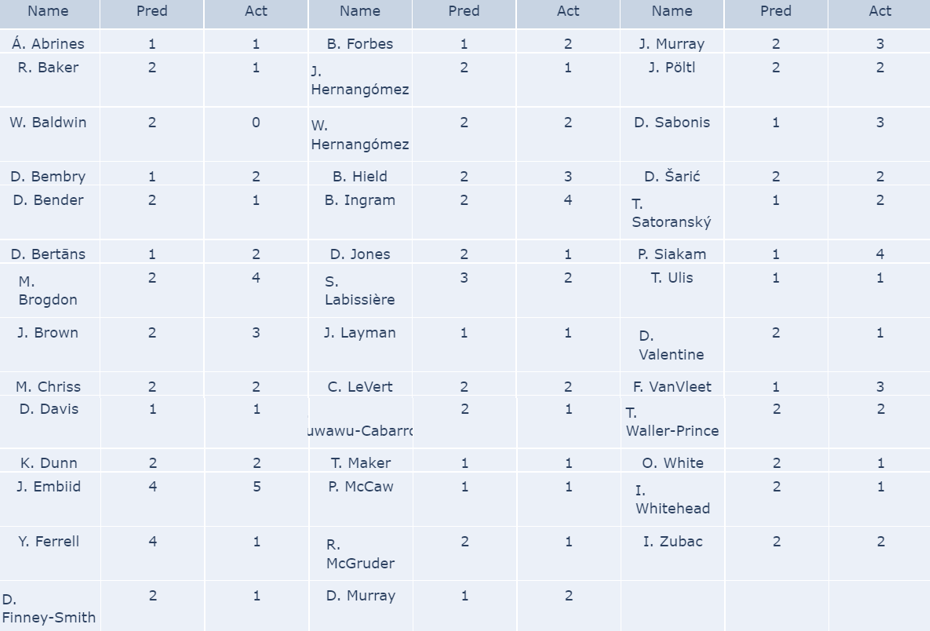
\includegraphics[width=12cm]{category_table17.PNG}
    \caption{Table showing the results of our ordinal classification on the 2016-2017 rookie dataset.}
\end{figure}

On average, our predictions were 0.878 tiers off, but this includes two big outliers. Pascal Siakam has progressed at an unprecedented rate since last year which leads to the model underestimating his 2019 NBA 2k rating. On the other hand, Yogi Ferrell was similar to Jahlil Okafor mentioned earlier in that he was in a system in which he got opportunities and his flaws were hidden early in his career, but he was soon found out to be a flawed player after his rookie season. However, even with these outliers, we still see pretty good predictions since we are not more than a tier away from the proper tier on average. This shows that this model does generalize to data it has not seen and can be used for future years as well.

\section{WMD and Fairness}
We do not believe that our work is a Weapon of Math Destruction. The models are easily testable since new 2K rankings are released every year and updated biweekly throughout the year. There are no real negative consequences to predictions either, other than perhaps players getting smaller contracts if NBA teams used these methods to predict future player worth. Even so, the average NBA salary is \$7.7 million and the median salary is \$3.5 million which means the consequences are hardly worthy of being considered dangerous or severely negative and fairness also becomes a non-issue. We also do not see self-fulfilling prophecies occurring as players can always outperform the model as proven by many positive outliers in our data like Pascal Siakam or Nikola Jokic.

\section{Summary}
Overall, both our regression and classification models were able to predict NBA 2K ratings 4 years down the line with reasonable accuracy. Both polynomial regression and ridge regression ended up with higher accuracy on the 2017 rookie test data than the data the models had actually trained on, while our classification-based approach ended up being a bit worse. One pattern we noticed throughout the process is that outliers were often "big-men" (tall players who play the power forward and center positions). These types of players are notoriously difficult to predict and can be seen as "boom or bust" prospects and that notion held true even in our purely objective analysis. In future work, perhaps we could add some kind of bias to help deal with this data. Despite these challenges, our overall accuracy makes us confident in using these models as a supporting tool to predict career trajectory, but we would not view them as a complete replacement for traditional methods.

\section{References}
\subsection{Python Libraries Used}
Scikit-learn: Machine Learning in Python, Pedregosa et al., JMLR 12, pp. 2825-2830, 2011.\\
\textit{Beautiful Soup}, https://pypi.org/project/beautifulsoup4/\\
\textit{Basketball Reference Web Scraper}, https://pypi.org/project/basketball-reference-web-scraper/
\subsection{Websites}
\textit{NBA 2K Ratings}, https://www.2kratings.com\\
\textit{Basketball Stats and History}, https://www.basketball-reference.com\\
\end{document}
